\documentclass[12pt, a4paper]{article}
\usepackage[a4paper, top=2cm, bottom=3cm, left=2cm, right=2cm]{geometry}
\usepackage[export]{adjustbox}
\usepackage{graphicx}
\usepackage{mathtools}
\usepackage{hyperref}
\usepackage{amsmath}
\usepackage{amsfonts}
\usepackage{amssymb}
\usepackage[version=4]{mhchem}
\usepackage{stmaryrd}
\usepackage{polyglossia}
\usepackage{fontspec}
\usepackage{ucharclasses}
\usepackage{fancyhdr}
\usepackage{wrapfig}
\usepackage{subcaption}
\usepackage{relsize}
\usepackage{framed}
\usepackage{changepage}
\usepackage{tabularray}
\usepackage{etoolbox}
\usepackage{xstring}
\usepackage{pstricks-add}
\usepackage{tikz}
\usepackage{empheq}
\usepackage{tcolorbox}
\usepackage[european,s traightvoltages, americanresistor, americaninductors]{circuitikz}
\usepackage{pgfplots}
\usepackage{tikz-3dplot}

\usetikzlibrary{
	angles,
	arrows.meta,
	positioning,
	arrows,
	backgrounds,
	calc,
	decorations,
	decorations.markings,
	decorations.pathmorphing,
	fit,
	shapes.arrows,
	shapes.callouts,
	shapes.geometric,
	shapes.misc,
	snakes,
	quotes
}
\pgfplotsset{compat=1.18}
\hypersetup{colorlinks=true, linkcolor=blue, filecolor=magenta, urlcolor=cyan,}
\urlstyle{same}

\setmainlanguage{english}
\setotherlanguages{norwegian, arabic}
\newfontfamily\arabicfont{Noto Naskh Arabic}
% \newfontfamily\lgcfont{CMU Serif}

%%%%%%%%%% Fancy header %%%%%%%%%
\pagestyle{fancy}
\fancyhead[C]{}
\fancyfoot[C]{\medskip\thepage}
\renewcommand{\footrulewidth}{.4pt}
\renewcommand{\headrulewidth}{0pt}

\setlength{\headheight}{14.49998pt}
\addtolength{\topmargin}{-2.49998pt}

\newcommand{\figwidth}{8cm}
\newcommand{\floatfigwidth}{5cm}


%%%%%%%%%% Formatters & Layout %%%%%%%%%
\newcommand{\uprimary}[1]{
	\section*{\center \Huge \underline{#1}}
	\addcontentsline{toc}{section}{\protect\numberline{}#1}
}
\newcommand{\usecondary}[1]{
	\section*{\center \LARGE \underline{#1}}
	\addcontentsline{toc}{section}{\protect\numberline{}#1}
}
\newcommand{\usection}[1]{
	\section*{\LARGE #1}
	\addcontentsline{toc}{subsection}{\protect\numberline{}#1}
}
\newcommand{\usubsection}[1]{
	\section*{\Large #1}
	\addcontentsline{toc}{subsection}{\protect\numberline{}#1}
}
\newcommand{\ussubsection}[1]{
	\section*{\large #1}
	\addcontentsline{toc}{subsection}{\protect\numberline{}#1}
}
\newcommand{\ans}{\bigskip\underline{\textbf{Answer}}}
\newcommand{\ques}[1]{\noparindent\textbf{#1}\doparindent}
\newcommand{\rfloatingimg}[1]{
	\begin{wrapfigure}{r}{\floatfigwidth}
		\includegraphics[max width=\floatfigwidth]{#1}
	\end{wrapfigure}
}
\newcommand{\indentbox}[2]{
	\begin{adjustwidth}{#1}{0pt}
		#2
	\end{adjustwidth}
}
\newcommand{\qa}[3]{
	\noparindent
	\textbf{#1 #2}
	\indentbox{.76cm}{
		\ans
		#3
	}
	\vspace{.75cm}
}
\newcommand{\noskipqa}[2]{
	\noparindent
	\textbf{#1}
	\indentbox{.76cm}{
		\ans
		#2
	}
}
\newcommand{\eqnleft}[1]{
	\begin{flalign*}
		 & #1 &  &
	\end{flalign*}
}
\newcommand{\fullwidthimg}[1]{
	\begin{center}
		\includegraphics[max width=\textwidth]{#1}
	\end{center}
}
\newcommand{\uheading}[2]{
	\uprimary{Module - #1}
	\vspace{-.7cm}
	\usecondary{#2}
}

\newcommand{\note}[1]{
	\begin{tcolorbox}[colframe=green!40!black, colback=green!5!white, title={\textbf{Note}}]
	#1
	\end{tcolorbox}
}


%%%%%%%%%% general constants/symbols %%%%%%%%%
\newcommand\longUparrow{\mathrel{\scalebox{1}[2]{$\uparrow$}}}
\DeclareRobustCommand{\rchi}{{\mathpalette\irchi\relax}}
\newcommand{\irchi}[2]{\raisebox{\depth}{$#1\chi$}}
\newcommand{\term}[1]{\underline{\textbf{#1}}}
\newcommand{\amstr}{\mathring{\textrm{A}}}
\newcommand{\h}{6.626 \times 10^{-34}}
\newcommand{\kB}{1.38 \times 10^{-23}}
\newcommand{\lc}{3 \times 10^{8}}
\newcommand{\uunit}[1]{\mathrm{~#1}}

%%%%%%%%%% Format constants %%%%%%%%%
\newcommand{\doparindent}{\setlength\parindent{.5cm}}
\newcommand{\noparindent}{\setlength\parindent{0pt}}
\graphicspath{ {../images/} }
\NewDocumentCommand{\multiskip}{m}{%
	\begingroup
	\newcount\i  % Define a new counter \i
	\i=0         % Initialize the counter
	\loop
	\ifnum\i<#1
	\bigskip  % Add \bigskip
	\advance\i by 1  % Increment the counter
	\repeat
	\endgroup
}

\newcommand{\termlist}[1]{
	\begin{tcolorbox}[colback=blue!10!white, colframe=blue!50!black, title={Some terms}]
		#1
	\end{tcolorbox}
}


%%%%% dev fx
% startx, starty, endx, endy
\newcommand{\dottedgrid}[4]{
	\draw[thin, dotted] (#1, #2) grid (#3,#4);
	\foreach \i in {#1,...,#3} \node at (\i,-2ex) {\i};
	\foreach \i in {#2,...,#4} \node at (-2ex,\i) {\i};
}
\newcommand{\smallmidarrow}[2]{\tikz \draw[arrows = {-Straight Barb[scale=.8]}, line width=#1] (0,0) -- +(#2,0);}
\newcommand{\midarrow}[2]{\tikz \draw[arrows = {-Straight Barb[scale=1.1]}, line width=#1] (0,0) -- +(#2,0);}

\DefTblrTemplate{caption-tag}{default}{}
\DefTblrTemplate{caption-sep}{default}{}
\DefTblrTemplate{caption-text}{default}{}
\DefTblrTemplate{contfoot-text}{default}{}
\DefTblrTemplate{conthead-text}{default}{}

\usepackage{tikz}
\usepackage{listofitems}
\usepackage{xargs}
\usepackage{fp}
\usetikzlibrary{3d,calc,patterns,quotes,angles,perspective}

\newcommandx{\shadedPlane}[6][5=blue, 6=0.8]{
	\readlist\a{#1}%
	\readlist\b{#2}%
	\readlist\c{#3}%
	\readlist\d{#4}%
	\coordinate (P1) at (\a[1], \a[2], \a[3]);
	\coordinate (P2) at (\b[1], \b[2], \b[3]);
	\coordinate (P3) at (\c[1], \c[2], \c[3]);
	\coordinate (P4) at (\d[1], \d[2], \d[3]);
	\fill[pattern=north east lines, pattern color=#5, opacity=#6]
	(P1) -- (P2) -- (P3) -- (P4)-- cycle;
	\draw[thick, color=#5, opacity=#6]
	(P1) -- (P2) -- (P3) -- (P4) -- cycle;
}

\newcommandx{\axes}[2][1=1, 2=1.3]{
	\FPeval\axside{#1 * #2}
	\draw[->, red] (0,0,0) -- (\axside,0,0) node[anchor=north east] {$x$};
	\draw[->, green] (0,0,0) -- (0,\axside,0) node[anchor=north west] {$y$};
	\draw[->, blue] (0,0,0) -- (0,0,\axside) node[anchor=south] {$z$};
}
\newcommandx{\wirecube}[2][2=1pt]{
	% vertices of the cube & plane
	\coordinate (A) at (0,0,0);
	\coordinate (B) at (#1,0,0);
	\coordinate (C) at (#1,#1,0);
	\coordinate (D) at (0,#1,0);
	\coordinate (E) at (0,0,#1);
	\coordinate (F) at (#1,0,#1);
	\coordinate (G) at (#1,#1,#1);
	\coordinate (H) at (0,#1,#1);

	% Draw the edges of the cube
	\draw[thick] (A) -- (B) -- (C) -- (D) -- cycle;
	\draw[thick] (E) -- (F) -- (G) -- (H) -- cycle;
	\draw[thick] (A) -- (E);
	\draw[thick] (B) -- (F);
	\draw[thick] (C) -- (G);
	\draw[thick] (D) -- (H);

	% Add points to illustrate vertices
	\foreach \i in {(A), (B), (C), (D), (E), (F), (G), (H)} {
			\filldraw[black] \i circle (#2);
		}
}

\newcommand{\wirecubewithlabels}[2]{
	\wirecube{#1}[#2]

	% Label the side lengths

	\coordinate (A) at (0,0,0);
	\coordinate (B) at (#1,0,0);
	\coordinate (D) at (0,#1,0);
	\coordinate (E) at (0,0,#1);

	\node at ($(A)!0.8!(B)$) [above] {$\vec{a}$};
	\node at ($(A)!0.7!(D)$) [above right] {$\vec{b}$};
	\node at ($(A)!0.7!(E)$) [above] {$\vec{c}$};
	\draw[thick, ->] (A) -- (B);
	\draw[thick, ->] (A) -- (D);
	\draw[thick, ->] (A) -- (E);
	\pic [blue,draw,angle radius=0.25cm] {angle=B--A--E};
	\pic [green,draw,angle radius=0.25cm] {angle=D--A--B};
	\pic [red,draw,angle radius=0.25cm] {angle=D--A--E};

	\node[color=blue, scale=.8] at (.4,0.4,0) {$\gamma$};
	\node[color=green, scale=.8] at (.7,0,.7) {$\beta$};
	\node[color=red, scale=.8] at (-0.3,0.3,0.3) {$\alpha$};
}

\newcommand{\smallmidarrow}[2]{\tikz \draw[arrows = {-Straight Barb[scale=.8]}, line width=#1] (0,0) -- +(#2,0);}
\newcommand{\midarrow}[2]{\tikz \draw[arrows = {-Straight Barb[scale=1.1]}, line width=#1] (0,0) -- +(#2,0);}
\newcommand{\millerDiagramQuad}[6]{
	\begin{tikzpicture}[
			scale=#6,
			x={(-.45cm, -.4cm)},
			y={(1cm, 0cm)},
			z={(0cm, 1cm)}
		]
		\axes[#5]
		\shadedPlane{#1}{#2}{#3}{#4}

		\wirecube{#5}[0pt]

	\end{tikzpicture}
}

\newcommand{\millerDiagram}[5]{
	\millerDiagramQuad{#1}{#2}{#3}{#3}{#4}{#5}
}

\newcommand{\doubleCylinder}[3]{
	\draw (0,0) ellipse (#1 and #1*2);
	\draw (0,#1*2) -- ++(#3, 0);
	\draw (0,-#1*2) -- ++(#3, 0);

	\draw (0,0) ellipse (#2 and #2*2);
	\draw (0,#2*2) -- ++(#3, 0);
	\draw (0,-#2*2) -- ++(#3, 0);
}

% x,y, r, y-scalar, x-length, y-shear, color
\newcommand{\cylinder}[7]{
	\begin{scope}[shift={(#1, #2)}]
		\draw[fill=#7, draw=black] (#5, #4*#3+#6) arc (90:-80:#3 and #4*#3) -- ++(-#5, -#6) arc (-80:90:#3 and #4*#3) -- cycle;
		\draw[fill=#7, draw=black] (0, 0) ellipse (#3 and #4*#3);
	\end{scope}
}

\begin{document}
\usection{Ordinary Differential Equations}
\usubsection{Introduction}
 6 Abstract of every vibration/flow is asmooth curve / diffeqn.

\begin{itemize}
  \item A carve can be represented as a function
  \item In $y=f(x), x$ is independent variable $\& y$ is a dependent variable
\end{itemize}

also in $z=f(x, y), x, y$ are independent variables \&

$z$ is dependent variable.

\section*{Differential equation}
An equation involving derivative(s) of dependent variable with respect to independent variable(s) is called differential equation.

$$
\text { e.g: } x \times \frac{d y}{d x}+y=0
$$

\section*{ODE}
A diffeq. involving depen derivortives of dependent variable with respect to only one independent variable

\begin{verbatim}
is
\end{verbatim}

\begin{itemize}
  \item only polyromial diff. gqs have degree
\end{itemize}

$$
3\left(\frac{d^{2} y}{d x^{2}}\right)^{4}+\left(\frac{d y}{d x}\right)^{5}=0
$$

degree 4

\begin{itemize}
  \item Order: Order of highest order derivutive of dependent variable, wrt. independent variable involved in the equation.
  \item Degree: If diffeqn. is a polynomial equation of derivative, the highest (power ( positive integral index) of highest order derivative is its degree.
\end{itemize}

creneral form: $f\left(x, y, y^{\prime}\right)=0$

$$
\begin{aligned}
& \text { or } y^{\prime}=g(x, y) \\
& \text { cy: } y^{2}=\sqrt{x^{2}+y^{2}}
\end{aligned}
$$

\section*{$1^{\text {st }}$ Order LDE}
$$
y^{\prime}+P(x) y=Q(x)
$$

: $p, q$ are continuous in same interval I

solution: $g(F)=\int Q \cdot(F) d x+C$ . $F=e^{\int P d x}$ Integration factor

$$
\text { 1. } y_{1}^{\prime}+2 x y=x
$$

A). Given is an $1^{\text {st }}$ order LDE

$$
\begin{array}{rlr}
P=2 x, Q=\infty, \\
\therefore F=e^{2} \int x \cdot d x=e^{x^{2}} \text { (integrating factor } \\
\therefore \text { Solution: } y \cdot e^{x^{2}}=\int x \cdot e^{x^{2}} d x+c & x^{2}= \\
& =\frac{1}{2} e^{x^{2}}+c & 2 x d x= \\
\therefore y=\frac{1}{2}+e^{-x^{2}} \cdot c & x \cdot d x
\end{array}
$$

\begin{enumerate}
  \setcounter{enumi}{1}
  \item Solve $\frac{d y}{d x}+2 y \tan (x)=\sin (x)$
\end{enumerate}

$$
\begin{aligned}
P(x) & =2 \tan (x), Q(x)=\sin (x) \\
I F & =e^{\int P \cdot d x} \\
& =e^{2 \cdot \ln |\sec (x)|} \\
& =|\sec (x)|^{2} \equiv \sec ^{2}(x)
\end{aligned}
$$

Solution $=y \cdot \sec ^{2}(x)=\int \sin (x) \cdot \sec ^{2}(x) d x+c$

$$
\begin{aligned}
& =\int \cdot \sec (x) \tan (x) d x+c \\
& =\sec (x)+c
\end{aligned}
$$

\section*{$y=\cos (x)+\cos ^{\circ 2}(x) \cdot c$}
\begin{enumerate}
  \setcounter{enumi}{2}
  \item Find solution of initial value problem:
\end{enumerate}

$$
x^{2} y^{\prime}-x y=x^{4} \cdot \cos (2 x), y(\pi)=2 \pi
$$

A $\quad x^{2} y^{\prime}-x y=x^{4} \cdot \cos (2 x)$

$\therefore y_{-}^{\prime}-x^{-1} y=x^{2} \cdot \cos (2 x)$

$\therefore P(x)=-x^{-1}, Q(x)=x^{2} \cdot \cos (2 x)$

$\therefore I F=e^{\int p(x) \cdot d x}=e^{-\int x^{-1} \cdot d x}=e^{-10[x]}=0\left(x^{2}\right)^{-1}$

$\therefore$ Solution: $y \cdot I F=\int Q \cdot I F \cdot d x+C$

$$
\begin{aligned}
y \cdot(x)^{-1} & =\int x^{2} \cdot(x)^{-1} \cdot \cos (2 x) \cdot d x+c \\
& =\int x \cdot \cos (2 x) d x+c \\
& =\frac{x x \cdot \sin (x)}{2}-\frac{1}{2} \int \sin (2 x) d x+c \\
& =\frac{x \sin (2 x)}{2}+\frac{\cos (2 x)}{4}+c \\
\therefore y & =\frac{x^{2} \cdot \sin (2 x)}{2}+\frac{x \cdot \cos (2 x)}{4}+x^{4} \cdot c
\end{aligned}
$$

I is given that $y(\pi)=2 \pi$

$$
\therefore 2 \pi=\frac{\pi^{2} \cdot \sin (2 \pi)}{2}+\frac{\pi \cdot \cos (2 \pi)}{4}+\pi \cdot c
$$

$$
\therefore 2=\frac{1}{4}+c \Rightarrow c=1 \frac{3}{4}=\frac{7}{4}
$$

Substitute in (2) to get specific solutions

$$
y=\frac{x^{2} \sin (2 x)}{2}+\frac{x \cdot \cos (2 x)}{4}+\frac{7}{4} x
$$

$$
\begin{aligned}
& 4 \text { Solve } y^{\prime}-2 x y=2 \\
& \text { 5. Solve } x y^{\prime}-2 y=-x \\
& G= \\
& 4 y^{\prime}-2 x y=2 x \\
& \text { Let } P(x)=-2 x, Q(x)=2 x \\
& I F=e^{\int F d x}=e^{\int-2 x \cdot d x}=e^{-x^{2}} \\
& \therefore \text { solution: } y \cdot e^{-x^{2}}=\int 2 x \cdot e^{-x^{2}} d x+c
\end{aligned}
$$

\begin{center}
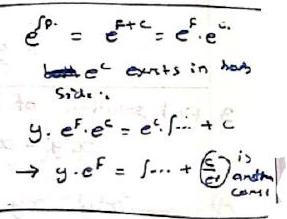
\includegraphics[max width=\textwidth]{2024_07_21_6c823ced6a9d46a245adg-1}
\end{center}

$$
\begin{aligned}
& \text { let }-x^{2}=t, \Rightarrow-2 x \cdot d x=d t \\
& \text { Put }-x^{2}=t \\
& \begin{aligned}
\therefore \int\left(2 x \cdot e^{-x^{2}} d x+c=-\int e^{t} d t\right. & =\frac{-e^{t}+0}{} \\
& =-e^{x^{2}}+
\end{aligned} \\
& -2 x d x=d A \\
& \therefore y=1+e^{x^{2}} \cdot c \\
& \int 2 x e^{-x^{2}} d x=-\int e^{t} d t \\
& \text { 5. } x y^{\prime}-2 y=-x \\
& \begin{array}{l}
=-e^{t} \\
=-e^{-n^{2}}
\end{array} \\
& \therefore y^{\prime}-2 x^{-1} \cdot y=- \\
& \therefore P(x)=-\frac{2}{x}, Q(x)=- \\
& \therefore I F=e^{\int A 1 x}=e^{-2 \int 1 / x \cdot d x}=e^{-2 \ln (x)}=x^{-2} \\
& y \cdot x^{-2}=\int x^{-2} \cdot-1+c \\
& =\frac{2^{-1}}{-1} \text { ar- }+c=\frac{1}{x}+c
\end{aligned}
$$

\section*{$\therefore y=x+c x^{2}$.}
\begin{enumerate}
  \setcounter{enumi}{5}
  \item $x y^{\prime}+2 y=\frac{\cos (x)}{x}$
\end{enumerate}

$y^{\prime}+\frac{2}{x} \cdot y=\frac{\cos (x)}{x^{2}}$

$P(x)=\frac{2}{x}, Q(x)=\frac{\cos (x)}{x^{2}}, I F=e^{\int p \cdot d x}=e^{\ln \left(x^{2}\right)}=x^{2}$ $y \cdot I F=\int I F \cdot Q \cdot d x+c$

$y \cdot x^{2}=\int x^{2} \cdot \frac{\cos (x)}{x^{2}} \cdot d x+c=\int \cos (x) d x+c$

$y \cdot x^{2}=\sin (x)+c \Rightarrow y=\frac{\sin (x)}{x^{2}}+\frac{c}{x^{2}}$

\begin{enumerate}
  \setcounter{enumi}{6}
  \item $y^{\prime}+\frac{2 y}{x}=\frac{4}{x}$,
\end{enumerate}

$P(x)=\frac{2}{x}, Q(x)=\frac{4}{x}, \quad$ F $=e^{\int P d x}=e^{2 \cdot \int 1 / x \cdot d x}=x^{2}$

$\therefore$ solution: $y \cdot x^{2}=\int x^{2} \cdot \frac{4}{x} d x+c=2 x^{2}+c$

$\cdots y=2+\frac{c}{x^{2}}$

Given $y(1)=6$,

$$
\therefore \quad 6=2+\frac{c}{1} \Rightarrow c=4
$$

$\therefore y=2+\frac{4}{x^{2}}$

Hw

$$
\begin{array}{ll}
\text { 1) }(x+1) y^{\prime}+2 y=(x+1)^{5 / 2} & \text { 2) } x y^{\prime}-2 y=x^{4} e^{x} \\
\text { 3) } x y^{\prime}-y=2 x \ln (x) & \text { 4) } y^{\prime}+y \cdot \tan (x)=\cos ^{2}(x) \\
\text { 5) } y^{\prime}+y \cdot \cot (x)=\csc ^{2}(x) & \text { 6) } x y^{\prime}+y=(1+x) e^{x} \\
\text { 7) } y^{\prime}+2 x y=x e^{-x^{2}} & \text { 8) } x y^{\prime}-2 y=x^{3} e^{x}, y(1)=0
\end{array}
$$

\section*{Variable Separable Equation}
A differential equation of the form ' $m(x, y) d x+n(x, y) d y=0$ ' is a variable separable equation if it can be expressed in the form: $f(x) d x+g(y) d y=0$

Solve : $\frac{d y}{d x}=\frac{y}{x}$

$d y \cdot x=d x \cdot y \rightarrow \frac{d x}{x}=\frac{d y}{y}$


$\ln (35)+c=\ln (x 0)+D$ $\therefore \ln (y)=\ln \operatorname{lse}+c+D$

$x_{y}=x \times e^{c+p} \ldots$ $3 x \sin (y) \cdot d x+\left(x^{2}+1\right) \cdot \cos (y) \cdot d y=0$

A) Divide by $\sin (y) \cdot\left(x^{2}+1\right)$

$$
\begin{aligned}
& \therefore \frac{x}{x^{2}+1} d x+\frac{\cos (y)}{\sin (y)} d y=0 \\
& \frac{1}{2} \int \frac{2 x \cdot d x}{x^{2}+1}+\int \frac{\cos (y)}{\sin (y)} d y=\ln (c)
\end{aligned}
$$

let $t=x^{2}+1, d x 2 x=d t$, let $u=\sin (y), \frac{d u}{d y}=\cos (y), d y \cdot \cos (y)=d u$

$\therefore \frac{1}{2} \int \frac{d t}{t}+\quad-\int \frac{d u}{u}=\ln (c)$

$=\frac{1}{2} \ln \left(x^{2}+1\right)+\ln (\sin (y))=\ln (c)$

$$
\begin{array}{r}
\ln \left[\frac{\left(x^{2}+1\right)^{2} \sin (y)}{c}\right]=0 \rightarrow \sin (y)=\frac{c}{\left(x^{2}+1\right)^{2}}, \\
y=\sin ^{-1}\left[\frac{c}{\left(x^{2}+1\right)^{2}}\right]
\end{array}
$$

\begin{enumerate}
  \setcounter{enumi}{3}
  \item $\tan (\theta) d r+2 r \cdot d \theta=0$
\end{enumerate}

$$
\begin{aligned}
& \frac{d r}{2 r}+\frac{d \theta}{\tan (\theta)}=0 \\
& \int \frac{d r}{2 r}+\int \underbrace{\int \frac{d \theta}{\tan (\theta)}}_{\operatorname{tat}(\theta) d \theta}=\ln (c) \\
& =\frac{1}{2} \ln (\gamma)+\ln (\sin (\theta))=\ln (c) \\
& =\ln (\sqrt{x})+\ln (\sin (\theta))=\ln (c) \\
& \ln (\sqrt{r})=\ln \left[\frac{c}{\sin (\theta)}\right] \\
& \sqrt{\gamma}=\sec \frac{c}{\sin (\theta)} \longrightarrow r \cdot \gamma \cdot \sin ^{2}(\theta)=c
\end{aligned}
$$

$4 x y d x+\left(x^{2}+1\right) d y=0$

$\rightarrow \frac{4 x}{x^{2}+1} d x+\frac{d y}{y}=0$

\begin{center}
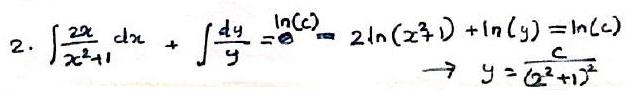
\includegraphics[max width=\textwidth]{2024_07_21_6c823ced6a9d46a245adg-2}
\end{center}

\section*{Homogenfous Differential Equation}
An differential equation that can be reduced into the form: $\frac{d y}{d x}=F\left(\frac{y}{x}\right)$ is called homogerious differential equation This can be solved by putting $y=v x$ and hence reducing to variable separable form.

\begin{enumerate}
  \item Solve $2 x y \cdot \frac{d y}{d x}-y^{2}+x^{2}=0$
\end{enumerate}

$$
2 x y \frac{d y}{d x}=y^{2}-x^{2} \Rightarrow \frac{d y}{d x}=\frac{y^{2}-x^{2}}{2 x y}-(1)
$$

pat $y=v x$ $v=\frac{y}{x}$

$$
\begin{aligned}
& \therefore(1) \equiv v+x \cdot \frac{d v}{d x}=\frac{v^{2} x^{2}-x^{2}}{2 x^{2} v}=\frac{\left(v^{2}-1\right)}{2 v}=\frac{\left(y^{2} / x^{2}-1\right)}{2 \cdot x / x x} \\
& x \cdot \frac{d v}{d x}=\frac{v^{2}-1}{2 v}-v=\frac{v^{2}-1-2 v^{2}}{2 v} \\
& x \cdot \frac{d v}{d x}=\frac{-\left(1+v^{2}\right)}{y v} \\
& \frac{2 v}{\left(c 1+v^{2}\right)} \cdot d v=\frac{d x}{x} \\
& \therefore-\int \frac{2 v}{\left(1+v^{2}\right)} d v=\int \frac{d x}{x}+\ln (c) \\
&=-\ln \left(v^{2}+1\right)=\ln (x)+\ln (c) \\
& x \equiv \ln \left(v^{2}+1\right)=-\ln (x)+\ln (c) \\
& \therefore v^{2}+1=\frac{c}{x} \\
& \frac{y^{2}}{x^{2}}+1=\frac{c}{x} \Rightarrow y^{2}+x^{2}=c x
\end{aligned}
$$

let $y=v x, \quad \therefore v=\frac{y}{x}$

$$
\therefore \frac{d y}{d x}=1+\frac{v x}{x}=1+v
$$

$=v+x \cdot \frac{d v}{d x}=1+v \Rightarrow x \cdot \frac{d v}{d x}=1 \Rightarrow \frac{d x}{x}=d v$

$$
\therefore \int \frac{d x}{x}=\int d v+c
$$

$$
=\ln (x)=v+c
$$

$$
y=\ln \left(\frac{x}{D}\right) \cdot x
$$

\section*{Bernoülli's Differential Equation}
A differential equation of form $y^{\prime}+p(x) y=Q(x) y^{n} . n \in \mathbb{R} /\{0,1\}$ called Bernocilli's Differential equation

Method to solve:

i.) Divide by $y^{n}$

$$
y^{-n} \cdot y^{\prime}+p(x) y^{1-n}=Q(x)-(1)
$$

\begin{enumerate}
  \setcounter{enumi}{1}
  \item put $z \leq y^{1-n}, \therefore \frac{d z}{d x}=(1-n) y^{-n} \cdot \frac{d y}{d x} \Rightarrow \underbrace{y^{-n} \cdot \frac{d y}{d x}=\frac{1}{1-n} \cdot \frac{d z}{d x}}_{\text {(2) }}$

  \item Substitute (2) in (1):

\end{enumerate}

$(1) \rightarrow \frac{1}{1-n} \cdot \frac{d z}{d x}+P(x) \cdot z=Q(x)$

$$
\Rightarrow z^{\prime}+(1-n) P(x) \cdot z=(1-n) Q(x)
$$

This is FLDE. in dependent variable $z$

$\therefore$ Solution:

$$
Z \cdot(I \cdot F)=\int(1-n) Q(x) \cdot I F \cdot d x+C \quad, I F=e^{\int(1-n) \cdot P(x) \cdot d x}
$$

Solve following:

a) $y^{\prime}+2 y=y^{2}$

A. Divide by $y^{2}$ :

$$
y^{-2} \cdot y^{\prime}+2 y^{-1}=1
$$

put $z=y^{-1} \quad \therefore z \frac{d z}{d x}=-y^{-2} \cdot \frac{d y}{d x}$

$\therefore$ (1) becomes:

$-\frac{d z}{d x}+2 z=1 \Rightarrow \frac{d z}{d x}-2 x=-1$

This is FLDE.

$\therefore P(x)=-2, \quad Q(x)=-1$

$I F=e^{\int P d x}=e^{\int-2 \cdot d x}=e^{-2 x}$

$\therefore$ General Solution:

$$
\begin{gathered}
\therefore z \cdot e^{-2 x}=\int-e^{-2 x} d z+c / 2 \\
z x e^{-2 x}=\frac{1}{2} e^{-2 x}+\frac{c}{2} \\
\text { now } z=y^{-1} \\
\therefore \quad y^{-1} \cdot e^{-2 x}=\frac{1}{2} e^{-2 x}+\frac{c}{2} \\
\therefore y=\frac{2}{1+e^{2 x} \cdot c}
\end{gathered}
$$

Divide by $y^{4}$ :

$$
y^{-4} \cdot \frac{d y}{d x}-y^{-3} \cdot \tan (x)=\sec (x)-(1)
$$

let $z=y^{-3}, \quad \frac{d z}{d x}=-3 . y^{-4} \cdot \frac{d y}{d x}$

multiply $\theta$ by -3 \& substitute $\frac{d z}{d x}$

$$
+3, \quad z \tan (x)=-3 \sec (x)
$$

$$
\begin{aligned}
& \frac{d z}{d x} \\
& P(x)=3 \tan (x) \quad Q(x)=-3 \sec (x) \\
& I: F=e^{\int P \cdot d x}=e^{3 \int \tan x \cdot d x}=e^{\ln \left(\sec ^{3}(x)\right)}=\sec ^{3}(x)
\end{aligned}
$$

multiply (2) by I.F.

$\sec ^{3}(x) \cdot \frac{d z}{d x}+3 \cdot \tan (x) \cdot \sec ^{3}(x) z=-3 \sec ^{4}(x)$

Apply reverse product rule: $u v^{\prime}+v u^{\prime}=(4 v)^{\prime}$

$$
\Rightarrow \frac{d}{d x}\left(\sec ^{3}(x) \cdot z\right)=-3 \sec ^{4}(x)
$$

$\int s c .^{4} \rightarrow \int \operatorname{se}^{2} \cdot \operatorname{sc}^{2}$

Integrate both sides: $\rightarrow\left(1+t^{2}\right) s c^{2}$


\begin{equation*}
\sec ^{3}(x) \cdot z=-3 \int \sec ^{4}(x) \cdot d x+c \tag{x}
\end{equation*}


$=\int(1+\infty) d t$

$$
=-3\left[\tan (x)+\frac{\tan ^{3}(x)}{3}\right]+c
$$

$\Rightarrow \frac{\sec ^{3}(x)}{y^{3}}=-3 \tan (x)=\tan ^{3}(x)+c$

$\therefore y=\frac{1}{\operatorname{sos}^{5}(x) \cdot \sqrt[3]{-3 \tan (x)-\tan ^{3}(x)+c}}$

d) $\frac{d y}{d x}+\tan (x) \tan (y)=\cos (x) \cdot \sec (y)$

A) This is B.D.E.

Divide by $\sec (y)$

$\cos (y) \frac{d y}{d x}+\tan (x) \sin (y)=\cos (x) \quad-(1)$

let $z=\sin (y) . \quad \frac{d z}{d x}=\cos (y) \cdot \frac{d y}{d x}$.

Substitute this in (1)

$\frac{d z}{d x}+\tan (x) \cdot z=\cos (x)$

let IF $=e^{\int \tan (x) \cdot d x}=e^{\ln (\sec (z))}=\sec (x)$

multiply both sides by T.F.

$\sec (x) \cdot \frac{d z}{d x}+\tan (x) \cdot \sec (x) \cdot z \cdot=1$

$\equiv \frac{d}{d x}(\sec (x) \cdot z)=1 \quad \Rightarrow \quad \sec (x) \cdot z=x+c \Rightarrow \sec (x) \cdot \sin (y)=x+c$.

$\therefore y=\sin ^{-1}(\cos (x) \cdot(x+c))$\\
d) $\frac{d y}{d x}+x \cdot \sin (2 y)=x^{3} \cdot \cos ^{2}(y)$

Divide by $\cos ^{2}(y)$ :

$\sec ^{2}(y) \cdot \frac{d y}{d x}+\frac{x \cdot 2 \sin (y) \cos (y)}{\cos ^{2}(y)}=x^{3}$

$\sec ^{2}(y) \frac{d y}{d x}+2 x \cdot \tan (y)=x^{3} \quad-10$

let $z=\tan (y) \quad \frac{d y}{d x}=\sec ^{2}(y) \cdot \frac{d y}{d x}$

substitute this in (1):

$\frac{d z}{d x}+2 x \cdot z=x^{3}$\\
let I.F $e^{\sqrt{2 x} \cdot d x}=e^{x^{2}}$, demultiply both sides by I.F $e^{x^{2}} \cdot \frac{d z}{d x}+z \cdot 2 x \cdot e^{x^{2}}=x^{3} e^{x^{2}}$

$\Rightarrow \frac{d}{d x}\left(e^{x^{2}} \cdot z\right)=x^{3} \varepsilon e^{x^{2}}$

\begin{center}
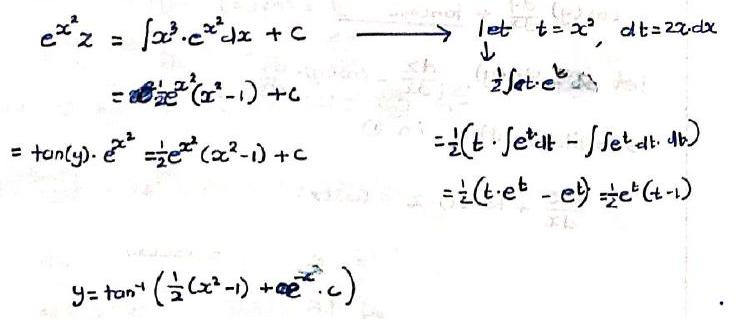
\includegraphics[max width=\textwidth]{2024_07_21_6c823ced6a9d46a245adg-4}
\end{center}

\section*{1.) $\frac{d y}{d x}+y=x y^{3} \quad$ 2) $\frac{d y}{d x}-y \tan (x)=y^{2} \cdot \sec (x)$ \\
 3) $\frac{d y}{d x}+\frac{y}{x}=\frac{y^{2}}{x} \ln (x)$ \\
 4) $\frac{d y}{d x}+x y=x^{3} y^{3}$}
\section*{Partial Differentiation}
If $z=f(x, y)$ it can be differentiated partially wort $x$ ory $\frac{\partial z}{\partial x}=\lim _{\Delta x \rightarrow 0} \frac{f(x+\Delta x, y)-f(x, y)}{\Delta x}$, Here we treat $y$ as constant $z_{x}=\frac{\partial z}{\partial x}$

e.y: $z(x, y)=x^{2}+y^{2}+2 x y$,

$z_{y}=\frac{\partial z}{\partial x}$ $\frac{\partial z}{\partial x}=2 x+0+2 y \quad 0$

or wirt. $y$ by: $\frac{\partial z}{\partial y}=\lim _{\Delta y \rightarrow 0} \frac{f(x, y+\Delta y)-f(x, y)}{\Delta y}$ [we treat $x$ constaint] $\frac{\partial z}{\partial y}=0+2 y+2 x$

find $\frac{\partial f}{\partial x} \& \frac{\partial f}{\partial y}$ in following:\\
a) $f(x, y)=x^{3}+3 x^{2} y+x y^{3}$\\
A) $\frac{\partial f}{\partial x}=3 x^{2}+6 x y+y^{3} \quad, \frac{\partial f}{\partial y}=0+3 x^{2}+3 x y^{2}$\\
b) $f(x, y)=2 x \cos (y)+3 x^{2} y$\\
A) $\frac{\partial f}{\partial x}=2 \cos (y)+6 x y \quad \frac{\partial f}{\partial y}=-2 x \sin (y)+3 x^{2}$

$$
\text { c) } \begin{aligned}
f(x, y) & =x \tan ^{-1}\left(\frac{y}{x}\right) \\
f_{x} & =\frac{1}{1+y^{2} / x^{2}} \cdot \frac{\partial}{\partial x} \cdot\left(\frac{y}{x}\right)=\frac{y}{x^{2}} \cdot \frac{x^{2}}{x^{2}+y^{2}} \cdot-\frac{1}{x^{2}}=\frac{-y}{x^{2}+y^{2}}
\end{aligned}
$$

$\Delta f_{y}=\frac{1}{1+y^{2} / x^{2}} \cdot \frac{\partial}{\partial y}\left(\frac{y}{x}\right)=\frac{x^{2}}{x^{2}+y^{2}} \cdot \frac{1}{x}=\frac{x}{x^{2}+y^{2}}$\\
d) $f(x, y)=x^{3}-x^{2} \sin (y)-y$

$f_{x}=3 x^{2}-2 x \sin (y) . \quad f_{y}=-x^{2} \cos (y)-1$

\section*{Higher Order Partial Derivative}
\begin{itemize}
  \item $\frac{\partial^{2} f}{\partial x^{2}}=\frac{\partial}{\partial x}\left(\frac{\partial f}{\partial x}\right)=f_{x x}$
  \item $\frac{\partial^{2} f}{\partial y^{2}}=\frac{\partial}{\partial y}\left(\frac{\partial f}{\partial y}\right)=f_{y y}$
\end{itemize}

$\cdot \frac{\partial^{2} f}{\partial x \partial y}=\frac{\partial}{\partial x}\left(\frac{\partial f}{\partial y}\right)=f_{x y}$

\begin{itemize}
  \item $\frac{\partial^{2} f}{\partial y \partial x}=\frac{\partial}{\partial y}\left(\frac{\partial f}{\partial x}\right)=f_{y x}$
\end{itemize}

\begin{itemize}
  \item If $f(x, y)$ is continuous function, $f_{x y}=f_{y x}$
\end{itemize}

\begin{enumerate}
  \item find I \& II order partial derivatives of\\
a) $t=x^{2} y$\\
A) $f_{x}=2 x y$. $f_{y}=x^{2}, f_{x y}=2 x, f_{y x}=2 x, f_{x x}=2 y, f_{y y}=0$\\
b) $x^{3} f(x, y)=x^{3} \sin (y)$
\end{enumerate}

$f_{x}=3 x^{2} \sin (y), f_{x x}=6 x \sin (y), f_{y x}=3 x^{2} \cos (y)$

$f_{y}=x^{3} \cos (y), \quad f_{y y}=-x^{3} \sin (y), \quad f_{x y}=-3 x^{2} \sin (y)$

\section*{Differentials}
If $z=f(x, y), d z, d x, d y$ are known as differentials. in $z, z, y$ respectively.

cex $d z=\frac{\partial z}{\partial x} d x+\frac{\partial z}{\partial y} d y$

1.) find the differentiols in $f$ of if $f=\frac{x^{3}}{3}-x y^{2}$

$$
\begin{array}{r}
d f=\frac{d f}{\partial x} \frac{\partial f}{\partial x} d x+\frac{\partial f}{\partial y} d y \\
d f=\left(x^{2}-y^{2}\right) d x-2 x y d y
\end{array}
$$

\section*{Exact Differential Equation}
\begin{itemize}
  \item A Differential equation of the form $M(x, y) d x+N(x, y) d y=0$ is sard to be exact differential equation.
\end{itemize}

such that $\frac{\partial \mu}{\partial x}=m(x, y), \& \frac{\partial \mu}{\partial y}=N(x, y)$

ie, $M d x+N d y=\frac{\partial \mu}{\partial x} d x+\frac{\partial \mu}{\partial y} d y=d \mu$

$$
\therefore \text { Solution is } \int d \mu \Rightarrow \mu(x, y)=c
$$

Methnd to find exact or not

\begin{itemize}
  \item If Diff. eqn. is exact then $\frac{\partial M}{\partial y}=\frac{\partial N}{\partial x}$
\end{itemize}

eg: $(1-x) \cdot d x-(1+y) d y=0$

$M=1-x, \quad N=-(1+y)$

$\frac{\partial M}{\partial y}=0, \quad \frac{\partial N}{\partial x}=0 \quad \Rightarrow \frac{\partial M}{\partial y}=\frac{\partial N}{\partial x} \quad \therefore$ Eqn. is exact.

Method to solve E.D.E

Solution: $\int M d x+\int[$ Terms in $N$ not containing $x] d y=c$

Solve $(1-x) d g-(1+y) d y=0$

A) Solution: $\int(1-x) d x+\int-(1+y) d y=c / 2 \quad$ (soy $)$

$$
\begin{gathered}
x-\frac{x^{2}}{2}-y-\frac{y^{2}}{2}=c / 2 \\
\Rightarrow \quad x-y=\frac{x^{2}+y^{2}}{2}+c / 2 \\
2(x-y)=x^{2}+y^{2}+c
\end{gathered}
$$

\begin{enumerate}
  \setcounter{enumi}{1}
  \item $\left(3 x^{2}+4 x y\right) d x+\left(2 x^{2}+2 y\right) d y=0$
\end{enumerate}

$$
\begin{aligned}
& M=3 x^{2}+4 x y, \quad \frac{\partial M}{\partial y}=4 x \\
& N=2 x^{2}+2 y \quad, \quad \frac{\partial N}{\partial x}=4 x \quad \frac{\partial M}{\partial y}=\frac{\partial N}{\partial x} \Rightarrow \text { eqn. is Exact }
\end{aligned}
$$

Solution: $\int M \cdot d x+\int[$ terms in $N$ not containing $x] d y=c$

$$
\begin{gathered}
\int\left(3 x^{2}+4 x y\right) d x+\int 2 y \cdot d y=c \\
x^{3}+2 x^{2} y+y^{2}=c
\end{gathered}
$$

\begin{enumerate}
  \setcounter{enumi}{2}
  \item Why condition for exactness is $\frac{\partial M}{\partial x}=\frac{\partial N}{\partial y}$ ?
\end{enumerate}

A) for \href{http://E.DE}{E.DE}. $\exists u(x, y): \frac{\partial u}{\partial y}=N(x, y) \cdot \frac{\partial u}{\partial x}=m(x, y)$

consider $\frac{\partial^{2} u}{\partial x \partial y}=\frac{\partial N}{\partial x}, \quad \frac{\partial^{2} u}{\partial y \partial x}=\frac{\partial M}{\partial y}$

since. $u(x, y)$ represents a family of curve and

it is continuous, $\frac{\partial^{2} u}{\partial x \partial y}=\frac{\partial^{2} u}{\partial y \partial x} \Rightarrow \frac{\partial M}{\partial y}=\frac{\partial N}{\partial x}$

\begin{enumerate}
  \setcounter{enumi}{1}
  \item Anodian woy]:
\end{enumerate}

$m=3 x^{2}+4 x y,(1) \quad N=2 x^{2}+2 y-(2)$

$\frac{\partial M}{\partial H}$ $=4 x$

$\nrightarrow \cdot m$ $0,4 x y+\Psi(x)$

$=4 x y+\psi(x)-15$

comparing (1) \& (3) $\psi(x)=3 x^{2}$

\begin{enumerate}
  \setcounter{enumi}{3}
  \item $\left(2 x \cos (y)+3 x^{2} y\right) d x+\left(x^{3}-x^{2} \sin y-y\right) d y=0$
\end{enumerate}

$$
\begin{array}{ll}
M=2 x \cos (y)+3 x^{2} y & N=x^{3}-x^{2} \sin (y)-y \\
\frac{\partial M}{\partial y}=-2 x \sin (y)+3 x^{2}, & \frac{\partial N}{\partial x}=3 x^{2}-2 x \sin (y) \\
\frac{\partial M}{\partial y}=\frac{\partial N}{\partial x} \Rightarrow \text { eqn. is EDE }
\end{array}
$$

Solution: $\int\left(2 x \cos (y)+3 x^{2} y\right) d x+\int-y d y \pm c$

$$
x^{2} \cos (y)+x^{3} y-\frac{y^{2}}{2}=c
$$

Hw:

\begin{enumerate}
  \item Solve:
\end{enumerate}

$$
\begin{aligned}
& \text { a) }\left(5 x^{4}+3 x^{2} y^{2}-2 x y^{3}\right) d x+\left(2 x^{3} y-3 x^{2} y^{2}-5 y^{4}\right) d y=0 \\
& \text { b) }(2 x y+y-\tan (y)) d x+\left(x^{2}-x \tan ^{2}(y)+\sec ^{2}(y)+2 y\right) d y=0
\end{aligned}
$$

\begin{enumerate}
  \setcounter{enumi}{1}
  \item (another uy).
\end{enumerate}

$$
M=3 x^{2}+4 x y, N=2 x^{2}+2 y
$$

Define $f(x, y)$ f $f_{x}=m . f_{y}=N$

Then solution is given by $f(x, y)=c_{1}$

\begin{enumerate}
  \item Integrate $f_{x}$ \href{http://wrt.ge}{wrt.ge} to find $f(x, y)$ :
\end{enumerate}

$$
f(x, y)=\int\left(3 x^{2}+4 y x\right) d x=x^{3}+2 x^{2} y+\psi(y) \quad
$$

Differentiate this curty to find $\psi(y)$ :

$$
\partial f_{y}=2 x^{2}+\frac{d \psi}{d y}
$$

Substitute $f_{y}=N, \quad$ (by $\left.d e f.\right)$

$$
2 x^{2}+\frac{d \psi}{d y}=2 x^{2}+2 y \Rightarrow \frac{d \psi}{d y}=2 y
$$

Integrate $d \psi$ sixy urty: $\psi(y)=y^{2}$

substitute $\psi(y)$ in $f(x, y)$ :

$$
f(x, y)=x^{3}+y^{2}+2 x^{2} y
$$

The Solution is $f(x, y)=c$ :

$$
\begin{gathered}
: \frac{x^{3}+y^{2}+2 x^{2} y=c}{2} \\
x^{4}+y^{2}+2 x^{2} y=x^{4}-x^{3}+c \\
\Rightarrow\left(y+x^{2}\right)^{2}=x^{4}-x^{3}+c \\
y+x^{2}= \pm \sqrt{x^{4}+x^{3}+c} \\
y=-x^{2} \pm \sqrt{x^{4}-x^{3}+c}
\end{gathered}
$$


$? \frac{d y^{4}}{d x}+\frac{x y}{1-x^{2}}=x \sqrt{y}$

divide by $\sqrt{y}$.


\begin{equation*}
y^{-1 / 2} \frac{d y}{d x}+\frac{x y^{1 / 2}}{1-x^{2}}=x \tag{1}
\end{equation*}


let $z=y^{1 / 2}, \quad \frac{d z}{d x}=\frac{1}{2} y^{-1 / 2} \frac{d y}{d x}$

$\therefore$ (1) become:

$$
\frac{d z}{d x}+\underbrace{\frac{d x}{2\left(1-x^{2}\right)}}_{p} \cdot z=\frac{1}{2} x \text {. }
$$

let $f=e^{\frac{1}{e} \int \frac{x}{1-x^{2}} d x}=\left(1-x^{2}\right)^{-1 / 4} \quad-\frac{1}{2} \int \frac{x}{1-x^{2}} d x$ $t=1-x^{2}$ $d t=d x \cdot(-2 x)$


\begin{align*}
s: \mathbb{Z} \cdot F=\int Q \cdot F \cdot d x+c & =-2 x \cdot d x \\
\Psi \cdot\left(1-x^{2}\right)^{-1 / 4} & =\int \frac{1}{2} x \cdot\left(1-x^{2}\right)^{-1 / 4} d x+c \quad-\frac{1}{4} \int \frac{d t}{t} \Rightarrow \Rightarrow n(t) \\
& =\quad \frac{1}{2} \int x \cdot\left(1-x^{2}\right)^{-1 / 4} d x+c \quad \text { - (2) }
\end{align*}


$\therefore$ Solution is: $y \cdot F=\int Q \cdot F \cdot d x+c$

let $t=1-x^{2}, d t=-2 x d x$

$\therefore$ (2) becomes:

$$
\begin{aligned}
y \cdot\left(1-x^{2}\right)^{-1 / 4} & =-\frac{1}{4} \int t^{-1 / 4} d t+c \\
& =-\frac{1}{4} x \frac{t^{3 / 4}}{-1 / 4+1}=-\frac{1}{3} \cdot t^{3 / 4}+c \\
z \cdot\left(1-x^{2}\right)^{-1 / 4} & =-\frac{1}{3}\left(1-x^{2}\right)^{3 / 4}+c \\
z & =-\frac{1}{3}\left(1-x^{2}\right)+c \cdot\left(1-x^{2}\right)^{1 / 4}
\end{aligned}
$$

$$
\begin{gathered}
z=\sqrt{y} \\
\therefore y=\left[\sqrt[4]{c \cdot\left(1-x^{2}\right)}-\frac{1}{3}\left(1-x^{2}\right)\right]^{2} \\
\frac{d y}{d x}+x \cdot \sin (2 y)=x^{3} \cdot \cos ^{2}(y) \\
\equiv \frac{d y}{d x}+x \cdot 2 \cdot \sin (y) \cos (y)=x^{3} \cdot \cos ^{2}(y)
\end{gathered}
$$

Divide by $\cos ^{2}(y)$ :

$$
\sec ^{2}(y) \cdot \frac{d y}{d x}+2 x \cdot \tan (y)=x^{3}
$$

let $z=\tan (y)=\frac{d z}{d x}=\sec ^{2}(y) \cdot \frac{d y}{d x}$.

$$
\frac{d z}{d x}+2 x \cdot z=x^{3}
$$

I.F $=e^{\sqrt{2 x}}=e^{x^{2}}$, \&multiply by it:

$$
\begin{aligned}
e^{x^{2}} \frac{d z}{d x} & +2 x \cdot e^{x^{2}} \cdot z=x^{3} \cdot e^{x^{2}} \\
\Rightarrow \quad e^{x^{2}} \cdot z & =\int x^{3} \cdot e^{x^{2}} d x^{+}+c \\
& =\frac{1}{2} e^{x^{2}}\left(x^{2}-1\right)+c \\
\therefore \tan (y) & =\frac{1}{2}\left(x^{2}-1\right)+e^{-x^{2}} \cdot c
\end{aligned}
$$

\begin{enumerate}
  \setcounter{enumi}{2}
  \item $\frac{d y}{d x}+y \tan (x)=y^{3} \cdot \sec (x)$
\end{enumerate}

EDE -Hw-1

$$
\begin{aligned}
& \underbrace{\left(5 x^{4}+3 x^{2} y^{2}-2 x y^{3}\right)}_{M} d x+\underbrace{\left(2 x^{3} y-3 x^{2} y^{2}-5 y^{4}\right)}_{N} d y=0 \\
& M_{x y}=6 x^{2} y-6 x y^{2}, N_{y}=6 x^{2} y-6 x y^{2} \\
& M_{y}=N_{y} \quad \therefore \text { EDE }
\end{aligned}
$$

$\therefore$ So ln: $\int_{\text {cor }} m d x+\int(N \not x) d x y=C$

$$
=x^{5}-y^{5}+x^{3} y^{2}-x^{2} y^{3}=c
$$

$29 / 9$

$$
\left(3 x^{2}+6 x y^{2}\right) d x+\left(6 x^{2} y+4 y^{3}\right) d y=0
$$

Solve:\\
a) $[\cos (x) \tan (y)+\cos (x+y)] d x+\left[\sin (x) \cdot \sec ^{2}(y)+\cos (x+y)\right] d y=0$\\
A) $M=\cos (x) \tan (y)+\cos (x+y) \cdot \frac{\partial M}{\partial y}=\cos (x) \cdot \sec ^{2}(y)-\sin (x+y)$

$$
N=\sin (x) \sec ^{2}(y)+\cos (x+y), \frac{\partial N}{\partial x}=\sec ^{2}(y) \cdot \cos (x)-\sin (x+y)
$$

$\frac{\partial M}{\partial y}=\frac{\partial r}{\partial x} \Rightarrow$ Equation is exact.

$\therefore$ Solution is:

$$
\begin{aligned}
& \int_{y \cdot \text { cons }} M \cdot d x+\underbrace{\int(\operatorname{tem} s \operatorname{in} N \text { not containing } x) d y}_{0} d=c \\
& \tan (y) \int \cos (x) d x+\int \cos (x+y) d x \quad=c \\
& \tan (y) \cdot \sin (x)+\sin (x+y)=c
\end{aligned}
$$

\begin{enumerate}
  \item $(y \cos (x)+1) d x+\sin (x) d y=0$

  \item $\left(\sec (x) \tan (x) \tan (y)-e^{x}\right) d x+\left(\sec (x) \sec ^{2}(y) d y=0\right.$

\end{enumerate}

Linear D.E with Constant Coeffis.

It is eqn of form.

$$
a_{0} \cdot \frac{d^{n} y}{d x^{n}}+a_{1} \frac{d^{n-1} y}{d x^{n-1}}+\cdots+a_{n-1} \frac{d y}{d x}+a_{n} y=\phi(x)
$$

where $a_{i} \in \mathbb{R}$,

If $\phi(x)=0$ : to solve this we have to change the equation to symbolic form. is $\left(a_{0} D^{n}+D a, D^{n-1}+\cdots\right) s=0 \$$ ItS Auxillary equation is: $\left(a_{\theta} m^{n}+a_{1} m^{n-1}+\cdots\right)$ ky $=0$

From the auxillory equation we get the roots, $m_{1}, m_{2}, \cdots$ Now we procede by following rales. (which depends on nature of roots.

\begin{center}
\begin{tabular}{|l|l|}
\hline
\multicolumn{1}{|c|}{Roots} & complimentary $f_{x}$ \\
\hline
1 Roots are Rd equal & $\left(c_{1}+c_{2} x\right) e^{m_{1} x}$ \\
$m_{1}=m_{2}$ & $c_{1} e^{m_{1} x}+c_{2} e^{m_{2} x}$ \\
$m_{1} \neq m_{2}$ &  \\
2) $m_{1}=m_{2}=m_{3}$ & $\left(c_{1}+c_{2} x+c_{3} x^{2}\right) e^{m_{1} x}$ \\
3) $m_{1} \neq m_{2} \neq m_{3}$. & $\left(c_{1} e^{m_{1} x}+c_{2} e^{m_{2} x}+c_{3} e_{3} x\right.$ \\
$4) m_{1}=m_{2} \neq m_{3}$ & $\left(c_{1}+c_{2} 2 e^{m_{1} x}+c_{3} e^{m_{3} x}\right.$ \\
4) $\mathbb{I}: \alpha \pm i \beta$ & $e^{\alpha x}\left(c_{1} \cos (\beta x)+c_{2} \sin (\beta x)\right)$ \\
\hline
\end{tabular}
\end{center}

\begin{itemize}
  \item From the nature of roots, we get complimentary function, Hence the Solution is:
\end{itemize}

$$
y=C \cdot F
$$

\begin{enumerate}
  \item Solve $\frac{d^{2} y}{d x}+\frac{\int}{d x}+6 y=0$
\end{enumerate}

Symbolic form: $\left(D^{2}+5 D+6\right) y=0 \Rightarrow(D+3)(D+2)=0$

$\therefore$ roots are: $m=-3,-2$

Real \& distinct.

$\therefore$ complimentary function is : $c_{1} \cdot e^{m \cdot x}+c_{2} \cdot e^{m_{2} x}$

$$
=c_{1} e^{-2 x}+c_{2} e^{-3 x}
$$

$\therefore$ Solution is: $\quad y=c_{1} e^{-2 x}+c_{2} e^{-3 x}$

2 Solve $\left(D^{3}+1\right) y=0$

$\rightarrow D^{3}=-1 \quad \Rightarrow \quad$ roots ar: $,-1, \frac{1}{2} \pm \frac{\sqrt{2}}{2} i$

usang: $(a+b)\left(a^{2}-a b+b^{2}\right)$

$$
\begin{aligned}
& \rightarrow(D+1)\left(D^{2}-D+1\right)=0 \\
& \Rightarrow \quad D+1=0 \Rightarrow \text { root }=-1 \\
& D^{2}-D+1=0 \Rightarrow \text { root }=\frac{1 \pm \sqrt{3} i}{2}
\end{aligned}
$$

$C F: \quad e^{1 / 2 x}\left(c_{1} \cos \left(\frac{\sqrt{3}}{2} x\right)+c_{2} \sin \left(\frac{\sqrt{3}}{2} x\right)\right)+c_{3} \cdot e^{-x}$\\
To find particular seder integral $\frac{\phi(e)}{5}$

Case

$$
I: \phi(x)=e^{a x}, \text { put } D=a
$$

e.g: $\frac{d^{2} y}{d x}-13 \frac{d y}{d x}+12 y=e^{-2 x}$

$$
\begin{aligned}
& \rightarrow \underbrace{\left(D^{2}-12 D+12\right) y}_{=0 \rightarrow \text { roots }}=e^{-2 x} \\
& \therefore C \cdot F=c_{1} e^{x}+c_{2} e^{12 x}
\end{aligned}
$$

$\therefore$ Porticulor integral $: P I=\frac{e^{-2 x}}{D^{2}-13 D+12} \quad, D=-2$,

$$
\Rightarrow \frac{e^{-2 x}}{4+26+12}=\frac{e^{-2 x}}{42}
$$

$\therefore$ Solution: $y=C F+P I$

$$
\begin{gathered}
\quad=c_{1} e^{x}+c_{2} e^{12 x}+\frac{e^{-2 x}}{42} \\
6 D^{2} y-D_{y}-2 y=e^{4 x} \quad, \quad 6 \\
\therefore \text { Auy-fx }=6 D^{2}-D-2, \text { rooks }=\frac{+1 \pm \sqrt{1+4 \times 6 \times 2}}{12}=\frac{1 \pm 7}{12} \Rightarrow \frac{2}{3}-\frac{1}{2} \\
\therefore C F=c_{1} e^{2 / 3 x}+c_{2} e^{1 / 2 x} \\
P I=\frac{e^{4 x}}{6 D^{2}-D-2}=\frac{e^{4 x}}{6 \times 16-4-2}=\frac{e^{4 x}}{90}
\end{gathered}
$$

$\therefore$ Solution:

$$
\begin{aligned}
& y=C F+P F \\
& =c_{1} e^{\frac{2}{3} x}+c_{2} e^{\frac{1}{2} x}+\frac{e^{4 x}}{90} \\
& y=c_{1}{\sqrt[3]{e^{x}}}^{2}+c_{2} \sqrt{e^{x}}+e^{4 x} / 90
\end{aligned}
$$

Particular Integral

case $2: \phi(x)=\cos (a x)$ or $\sin (a x)$, put $D^{2}=a-a^{2}$ ?. Solve $\left(0^{2}+4\right) y=\cos (3 x)$

Aux. $f_{x}=D^{2}+4$, roots $= \pm 2 i$

$\therefore C F=$ $e^{o x}\left(c_{1} \cdot \sin (2 x)+c_{2} \cdot \cos (2 x)\right)=c_{1} \cdot \sin (2 x)+c_{2} \cdot \cos (22)$

$P I=\frac{\cos (3 x)}{D^{2}+4}=\frac{\cos (3 x)}{-9+4}=\frac{\cos (3 x)}{-5}$

$\therefore y=C F+P I$

$=c_{1} \sin (2 x)+c_{2} \cdot \cos (2 x)-\frac{\cos (3 x)}{5}$

II? $\left(D^{2}-3 D+2\right) y=\sin (3 x)$

Aux. $f_{x}: D^{2}-3 D+2 \rightarrow$ routs $: 1,2$

$\therefore C F=c_{1} e^{x}+c_{2} e^{2 x}$

$D^{2}=-9$

$P I=\frac{\sin (3 x)}{D^{2}-3 D+2}=$

$$
\begin{aligned}
& =-\frac{\sin (3 x)}{67+3 D}=\frac{-\sin (52)}{3 D+7} \\
& =\frac{-\sin (3 x)(30-7)}{9 D^{2}-49} \\
& =\sin (3 x) \cdot(3 D-7) \\
& =+81+49 \\
& =\frac{\sin (3 x)(3 D-7)}{130} \\
& =\frac{1}{130}\left(\frac{3 D \cdot \sin (3 x)}{\frac{d \sin (x)}{d x}}-7 \cdot \sin (3 x)\right) \\
& =\frac{1}{130}(9 \cos (3 x)-7 \sin (30))
\end{aligned}
$$

$\therefore$ Solution: $c_{1} e^{x}+c_{2} e^{2 x}+\frac{1}{130}(9 \cos (3 x)-7 \sin (3 x))$

$\left(D^{2}-2 D-8\right) y=4 \cos (2 x)+e^{4 x}$

Aus. $f_{n}=D^{2}-2 D-8 \Rightarrow(D-4)(D+2) \Rightarrow$ roots $24,-2$,

$\therefore C \cdot F=c_{1} e^{4 x}+c_{2} e^{-2 x}$

$$
\begin{aligned}
& P I_{1}=\frac{4 \cos (2 x)}{D^{2}-2 D-8} \quad D^{2}=-4 \\
& =\frac{4 \cos (2 x)}{-4-2 D-8}=-\frac{4 \cos (2 x)}{-2 D+12} \\
& \Rightarrow \frac{-2 \cos (2 x)(D-6)}{(D+6)(D-6)}=\frac{-2 \cos (2 x)(D-6)}{D^{2}-36} \\
& \begin{aligned}
& =\frac{2 \cos (2 x)(D-6)}{40} \\
& =\frac{\cos (2 x)(D-6)}{20}
\end{aligned} \\
& =\frac{D \cdot \cos (2 x)-6 \cos (2 x)}{20} \\
& =-\frac{\sin (2 x)+3 \cos (2 x)}{10}
\end{aligned}
$$

$$
\begin{array}{rlrl}
P I_{2} & =\frac{e^{4 x}}{D^{2}-2 D-8} & D=4 \quad *: 1 f f(x)=e^{a x} \\
& =\frac{e^{4 x}}{16-8-8} \quad \frac{1}{f(a)}=0, \frac{1}{f(D)} e^{a x}=\frac{x}{\phi} \\
& =\frac{e^{4 x}}{0} & \frac{1}{0} \quad f(x)=\cos (a x) \& \frac{1}{f\left(\left(^{2}\right)\right.}=0
\end{array}
$$

$$
\begin{array}{rlrl}
P I_{2} & =\frac{e^{4 x}}{(D-4)(D+2)} & \text { * If } f(x)=\sin (a x) d \frac{1}{f\left(D^{2}\right)}=0 \\
& =\frac{1}{D-4} \times \frac{e^{4 x}}{D+2} & \frac{1}{f(D)} \sin (a x)=\frac{-x \cdot \cos (a x)}{29} \\
\Rightarrow & =\frac{x e^{4 x}}{4+2}=\frac{x e^{4 x}}{6}
\end{array}
$$

$\therefore$ Solution is: $C F+P I_{1}+P I_{2}$

$$
=c_{1} e^{4 x}+c_{2} e^{-2 x}-\frac{\sin (2 x)+3 \cos (2 x)}{10}+\frac{x e^{4 x}}{6}
$$

\begin{enumerate}
  \setcounter{enumi}{1}
  \item $\left(D^{2}-9\right) y=1+5 e^{4 x}+2 e^{3 x}$
\end{enumerate}

A)

$$
\begin{aligned}
\text { Aus } F_{n} & =D^{2}-9=3,-3 \\
C F & =c_{1} e^{3 x}+c_{2} e^{-3 x} \\
P I_{1} & =\frac{e^{0 x}}{D^{2}-9}=D^{2}=0 \\
& =\frac{1}{-9} \quad D=4 \\
P I_{2} & =\frac{5 e^{4 x}}{D^{2}-9} \quad \frac{5 e^{4 x}}{7}=\frac{1}{(D-3)} \cdot \frac{2 e^{3 x}}{(D+3)} \\
& =\frac{2 e^{3 x}}{D^{2}-9}=\frac{2 x e^{3 x}}{6}=\frac{x e^{3 x}}{3}
\end{aligned}
$$

$\therefore$ Solution: $c_{1} e^{3 x}+c_{2} e^{-3 x}-\frac{1}{9}+\frac{5 e^{4 x}}{7}+\frac{x e^{3 x}}{3}$\\
3. $\left(0^{2}+16\right) y=\cos (4 x)$

Case 3: $\phi(x)=x^{m}$

To find PI. $\frac{1}{f(D)} \phi(x)$, take $[f(D)]^{-1} \phi(x)$

$\rightarrow$ expand binomially, neglecting higher powers of $D$, (upto $m^{\text {th }}$ power)

$$
\begin{aligned}
& (1+x)^{n}=1+n x+\frac{n(n-1)}{2!} x^{2}+\frac{n(n-1)(n-2)}{3!} x^{3}+\cdots \\
& (1+x)^{-1}=1-x+x^{2}-x^{3}+x^{4}+\cdots \\
& (1+x)^{-2}=1-2 x+3 x^{2} 4-4 x^{3}+\cdots
\end{aligned}
$$

\begin{enumerate}
  \item $\left(D^{2}+D+1\right) y=x^{2}$
\end{enumerate}

Aux. $f$ n $=D^{2}+D+1$, roots: $\quad \frac{-1 \pm \sqrt{-3}}{2}=\frac{-1 \pm i \sqrt{3}}{2}$

$$
\begin{aligned}
E F= & e^{-\frac{1}{2} x}\left(C_{1} \cos (\sqrt{3} x)+C_{2} \sin (x \sqrt{3})\right) \\
P I=\frac{x^{2}}{D^{2}+D+1} & =\left(1+\left(D+D^{2}\right)\right)^{-1} x^{2} \\
& =\left(1-\left(D+D^{2}\right)+\left(D+D^{2}\right)^{2}-\left(D+D^{2}\right)^{3}+\cdots\right) x^{2} \\
& =\left[1-D-D^{2}+D^{2}+2 D^{3}+D^{4}\right] x^{2} \\
& =x^{2}-D\left(x^{2}\right)-D^{2}\left(x^{2}\right)+D^{2}\left(x^{2}\right)+2 D^{3}\left(x^{2}\right)+D^{4}\left(x^{2}\right) \\
& =x^{2}-D\left(x^{2}\right)+2 D^{3}\left(x^{2}\right)+D^{4}\left(x^{2}\right) \\
& =x^{2}-2 x+0+0=x^{2}-2 x
\end{aligned}
$$

$\therefore$ Solution: $y=c F+P I=e^{-\frac{1}{2} x}\left(c_{1} \cos (x \sqrt{3})+c_{2} \sin (x \sqrt{3})\right)+x^{2} \rightarrow-p$

$$
\begin{aligned}
& \left(D^{2}+2 D+1\right) y=2 x+x^{2} \\
& \quad-1 \\
& \quad \therefore F=c_{1} e^{-x}+c_{2} e^{-x} x
\end{aligned}
$$

$$
\begin{aligned}
& P I_{1}=\frac{2 x}{D^{2}+2 D+1}=\left(D^{2}+2 D+1\right)^{-1}(2 x) \\
& =(D+1)^{-2}(2 x) \\
& =\left(1-2 D+3 D^{2}\right) 2 x \\
& =1-2 D(2 x)+3 D^{2}(2 x) \\
& =2 x-4+6=2 x-4 \\
& P I_{2}=\frac{x^{2}}{(D+1)^{2}}=(D+1)^{-2}\left(x^{2}\right) \\
& =\left(1-2 D+3 D^{2}\right) x^{2} \\
& =x^{2}-2 D\left(x^{2}\right)+3 D^{2}\left(x^{2}\right) \\
& =x^{2}-4 x+6=x^{2}-4 x+6
\end{aligned}
$$

$$
\begin{aligned}
\therefore \text { Solution }=y & =c_{1} e^{-x}+x^{2} \nrightarrow-2 x+2+c_{1} e^{-x} \\
& =e^{-x}\left(c_{1}+c_{2} x\right)+x^{2}-2 x+2
\end{aligned}
$$

$$
\begin{array}{rlr}
\left(2 D^{2}-5 D+3\right) y & =\cos (3 x) \cos (2 x) & \\
& =\frac{1}{2}(\cos (5 x)-\cos (x)) & C_{H} C_{B} \\
2 D^{2}-5 D+3 & =\frac{5 \pm \sqrt{25-24}}{4} \Rightarrow \frac{3}{2}, 1 & S_{1} S_{2}= \\
\therefore C F & =C_{1} e^{3 / 2 x}+C_{2} e^{x} & S_{1} C_{2}= \\
P I_{1} & =\frac{1}{2} \frac{\cos (5 x)}{2 D^{2}-5 D+3} & C_{1}= \\
& =\frac{1}{2} \frac{\cos (5 x)}{10-5 D+3}=-\frac{1}{2} \frac{\cos (5 x)}{5 D-13}=\frac{1}{2} \frac{\cos (5 x)(5 D+13)}{25 D^{2}-16 q}
\end{array}
$$

$$
C_{A} C_{B}=\frac{1}{2}[C(A+B)+C(A-B)]
$$

$$
\begin{aligned}
&=-\frac{1}{2} \frac{\cos (5 x)(5 D+13)}{125-169}=\frac{\cos (58)(50+13)}{88} \\
&=\frac{5 D(\cos (5 x))+13 \cos (5 x)}{88} \\
&=\frac{13 \cos (5 x)-25 \sin (5 x)}{88} \\
& P I_{2}=\frac{1}{2} \frac{\cos (x)}{2 D^{2}-50+3} \xrightarrow[Z]{ }
\end{aligned}
$$

$\therefore$ solution: $C_{1} e^{3 / 2 x}+c_{2} e^{x}+\frac{1}{5668}(47 \cos (5 x)+25 \sin (5 x))$

$\left(D^{2}-4 D+3\right) y=\sin (3 x) \cos (2 x)$

A $2^{\text {nd }} O . D E$. has complimentary fo $\$$ particular integral compl.fn is of form: $A e^{m} x+B e^{m_{2} x}+B C e^{m} x \ldots$ where $m_{1}, m_{2}, m_{3}$ are roots of auzillory $f_{n}$. for imaginary roots:

let $a_{5 b i}$ be the root,

$\therefore$ Solution is: $A e^{(a+b i) x}+B e^{(a-b i) x}$

$$
\begin{aligned}
& \Rightarrow A e^{a x} e^{b i x}+B e^{a x} e^{-b i x} \\
& =e^{a x}\left(A e^{b i x}+B e^{-b i x}\right) \\
& =e^{a x}(A(\cos (b x)+i \sin (b x))+B(\cos (b x)-i \sin (b x)) \\
& =e^{a x}((A+B)(\cos (b x)+(A-B) i \sin (b x))
\end{aligned}
$$

$$
\begin{aligned}
& \begin{array}{l}
\rightarrow e^{a x}(c \cdot \cos (b x) \\
\sin (3 x) \cos (2 x)
\end{array} \\
& =\frac{1}{2} \sin (5 x)+\frac{1}{2} \sin ^{\sin }(x) \\
& \text { Aux. } f_{n}=D^{2}-4 D+3, \text { roots }=1,3 \\
& =(D-1)(D-3) \\
& \therefore C F=c_{1} e^{x}+c_{2} e^{3 x} \\
& P I_{1}=\frac{\sin (5 x)}{2\left(D^{2}-4 D+3\right)} \quad, D^{2}=5 \\
& \Rightarrow \frac{\sin (5 x)}{13-8 D} \Rightarrow \frac{\sin (5 x)(13+8 D)}{169-64 D^{2}}=-\frac{\sin (5 x)(13+8 D)}{151} \\
& =-\frac{13 \sin (5 x)-40 \cos (5 x)}{151} \\
& P I_{2}=\frac{\sin (x)}{2\left(D^{2}-4 D+3\right)} \Rightarrow C D^{2}=1 \\
& \Rightarrow \quad \frac{\sin (x)}{5-4 D} \Rightarrow \frac{\sin ^{2}(x)(5+4 D)}{25-160^{2}}=\frac{\sin (x)+4 \cos (x)}{9}
\end{aligned}
$$

$\therefore$ Solution: $y=C F+P I_{1}+P I_{2}$

$$
=c_{1} e^{x}+c_{2} e^{3 x}-\frac{13 \sin (5 x)+40 \cos (5 x)}{91}+\frac{5 \cos (x)-4 \sin (x)}{9}
$$

Case $\forall$ T $-e^{a x} f(x)$

$\lambda\left(D^{2}+30+2\right) y=e^{2 x} \sin (x)$

C.F in $y=c_{1} e^{-1}+c_{2} e^{-2 x}$

$$
P . I,=\frac{e^{2 x} \sin (x)}{D^{2}+3 x+2}=e^{2 x} \cdot \frac{\sin (x)}{D^{2}+3 D+2} \stackrel{D=D+a}{\sin (x)} \cdot e^{2 x}
$$

$$
\begin{aligned}
& \frac{\sin (x)}{D^{2}+4 D+4+3 D+6+2} e^{23} \\
& =\frac{\overline{\sin (x)}}{D^{2}+7 x+12} e^{2 x} \\
& D^{2}=-(1) \\
& \rightarrow \frac{\sin (x)}{70+11} e^{221} \\
& \Rightarrow \frac{\sin (x)(7 D \bar{a} 11)}{\cos D^{2}-121} e^{22} \\
& \Rightarrow \frac{\sin (x)(70-11)}{-170}\left(e^{2 x}\right) \Rightarrow \frac{7 \cos (x)-11 \cos \sin (x)}{9} \cdot e^{2 x}
\end{aligned}
$$

-Solution.

$$
y=c_{1} e^{-x}+c_{2} e^{-2 x}+\frac{11 \sin (x)-7 \cos (x)}{170} e^{2 x}
$$

Ho

$$
\left\{\begin{array}{l}
\left(D^{2}+4 D+5\right) y=12 e^{-12} \cdot \cos (x) \\
\left(D^{2}-2 D+1\right) y=x e^{2 x}
\end{array}\right.
$$

e.

$$
\therefore C F=c_{1} e^{-x}+c_{2} x e^{x}
$$

$$
\begin{aligned}
& \left.P I=e^{2 x} \cdot \frac{x}{D^{2}-2 D+1}=D^{2}\right\} \\
& y e^{2 x}-\left(D^{2}-2 D+1\right) x
\end{aligned}
$$

$$
\begin{aligned}
& \Rightarrow e^{2 x} \cdot\left(D^{2}-2 D+1\right)^{21} x \\
& \Rightarrow e^{2 x} \cdot(D-1)^{-2} \cdot x \\
& \Rightarrow e^{2 x} \cdot\left(1+2 D-3 D^{2}\right) x \\
& \Rightarrow e^{2 x} \cdot(x+2)
\end{aligned}
$$

$$
\begin{aligned}
\Rightarrow & \frac{x}{(D-1+2)^{2}} \cdot e^{2 x} \\
\Rightarrow & (D+1)^{-2} x \cdot e^{2 x} \\
& \left(1+2 D+3 D^{2}\right) x \cdot e^{2 x} \\
\Rightarrow & (x-2) e^{2 x}
\end{aligned}
$$

$\therefore$ Solution: $y=c_{1} e^{x}+c_{2} e^{x}+(x-2) e^{2 x}$


\begin{align*}
& \left(D^{3}-3 D_{x}^{2}+3 D-3\right) y=x^{2} e^{x} \\
& \Rightarrow(D-1)^{3} \Rightarrow D=1 \\
& \therefore \quad c=c_{1} e^{x}+c_{2} e^{x} \cdot x+c_{2} x^{2} e^{x} \\
& P I=e^{x} \cdot \frac{x^{2}}{(Q-1)^{3}}, \quad D \rightarrow D+1 \\
& \Rightarrow e^{x} \frac{x^{2}}{D^{3}} \Rightarrow e^{x} \cdot\left(D^{-3}\right) x^{2} \\
& e^{x} \cdot\left(D^{-2}\right) \frac{x^{3}}{3}=e^{x} \cdot\left(D^{-1} \cdot \frac{24}{12}\right)=e^{x} \cdot \frac{25}{650} \\
& D^{-3}+(D+1-1)^{-3} \rightarrow(1+(D-1))^{3} x^{2} \\
& \rightarrow\left(1+3(D-1)+3(D-1)^{2}\right) \gtrless^{2} \\
& =x^{2}+3(D-1) x^{2}+3\left(D^{2}-2 D+1\right) x^{2} \\
& \Rightarrow x^{2}+(3 D-3) x^{2}+\left(3 D^{2}-6 D+3\right) x^{2} \\
& \Rightarrow x^{2}+-3 x^{2}+6 \\
& x^{2}+6 x^{3}+6-12 x  \tag{1}\\
& \left(D^{2}-2 D+1\right) y=x \cdot e^{x} \sin (x) \\
& C \cdot f=\operatorname{se}\left(c_{1}+c_{2} x\right) e^{x} \\
& P I=e^{x} \cdot \frac{x \sin (x)}{(D-1)^{2}} \stackrel{D \rightarrow D+1}{2} e^{x} \cdot \frac{x \sin (x)}{D^{2}} \\
& =e^{x} \cdot D^{1}(x \cdot \sin (x))
\end{align*}


$$
\begin{aligned}
& e^{x} \cdot D^{-4}(-x \cdot \cos (x)+\sin (x)) \\
& e^{x} \cdot(-x \cdot \sin (x)+\cos (x)+\cos (x) \\
& \Rightarrow e^{x} \cdot(x \sin (x)+2 \cos (x)) \\
& \therefore \text { soln } \quad y=\left(c_{1}+c_{2} x-x \sin (x)-2 \cos (x)\right) e^{x}
\end{aligned}
$$

Cauchy's LDE

General form:

$$
a_{0} x^{n} \cdot \frac{d^{n} y}{d x^{n}}+a_{1} x^{n-1} \frac{d^{n-1} y}{d x^{n-1}}+\cdots+a_{x} x^{d y} d x+y=\phi(x)
$$

is reduced to LDE with Const. coett by substituting

$$
\begin{aligned}
& x=e^{t} \text {, or } t=\ln (x) \quad \frac{d}{d t}=D, \because x^{2} \cdot \frac{d^{2} y}{d x^{2}} \Rightarrow D(D-1) y \\
& x \frac{d y}{d x}=D y \quad: \quad x^{3} \frac{d^{3} y}{d x^{3}} \rightarrow D(D-1)(D-2) y
\end{aligned}
$$

Solve:

1). $x^{2} \cdot \frac{d^{2} y}{d x^{2}}-x \frac{d y}{d x}+y=\ln (x)$

This if Cauchy's LDG $\therefore$ put $x=e^{t}, \Rightarrow \sin (x)=t$

Redue to LDE with const-eoeth.

$$
\begin{aligned}
\text { (1) } \rightarrow & D(D-1) y-D y+y=t \\
& \left(D^{2}-2 D+1\right) y=t \\
& \therefore C F=\left(c_{1}+c_{2} t\right) e^{t}
\end{aligned}
$$

$$
\begin{aligned}
& P_{I}=\frac{t}{(D-1)^{2}} \rightarrow \\
&= \frac{t}{D^{2}-2 D+1}=\left(1+\left(D^{2}-2 D\right)\right)^{-2}= \\
&=\left(1-D^{2}+2 D\right) t \\
&=t+2 \\
&=\ln (x)+2
\end{aligned}
$$

$\therefore$ solution: $y=\left(c_{1}+c_{2} \ln (x)\right) e^{\ln (x)}+\ln (x)+2$

$$
\begin{aligned}
& \left.=\oint_{1}+r_{2} \ln (x)\right] x+\ln (x)+2 \\
& =c_{1} x+\ln (x)\left(1+x c_{2}\right)+2
\end{aligned}
$$

\begin{enumerate}
  \setcounter{enumi}{1}
  \item $x^{2} \cdot y^{\prime \prime}-4 x y^{\prime}+6 y=x^{2}$
\end{enumerate}

put $x=e^{t}, t=\ln (x)$

$$
\begin{aligned}
& D(D-1) y-4 D y+6 y=e^{2 t} \\
& \left(D^{2}-5 D+6\right) y=e^{2 t} \\
& D=\frac{e^{2 t}}{D^{2}-5 D+6}, \quad C F=c_{1} e^{+3 x}+c_{2} e^{-12 x} \\
& \therefore P I_{1}=2 \\
& \Rightarrow \frac{e^{2 t}}{4-10+6}=
\end{aligned}
$$

$$
\begin{aligned}
& \frac{+5 \pm \sqrt{25-25}}{2}=\frac{+5 \pm 1}{2} \\
& =+2,-3 \\
& \frac{e^{2 t}}{(D-3)(D-2)} \Rightarrow \frac{1}{D-2} \cdot \frac{t e^{2 t}}{D-3}=-t e^{2 t}
\end{aligned}
$$

$\therefore$ Solution: $y=c_{1} e^{3 t}+c_{2} e^{2 t}+t e^{2 t}$

$$
=c_{1} e^{\ln (x)^{2}}+c_{2} e^{2 \cdot \ln (x)}-\ln (x) e^{2 \ln (x)}
$$

$$
\begin{aligned}
& =c_{1} x^{3}+c_{2} x^{2}-\ln (x) x^{2} \\
y & =c_{1} x^{3}+x^{2}\left(c_{2}-\ln (x)\right)
\end{aligned}
$$

HT\\
3. $x^{2} y^{\prime \prime}-2 x y^{\prime}-4 y=x^{4}$.\\
4. $x^{2} y^{\prime \prime}+4 x y^{\prime}+2 y=x^{2}+x^{-2}$

In 10\\
H.

Simultaneous LDE

It contains two or more dependent variables (soy $x, y .$. and one inclependent variable (say $t$ )

\begin{enumerate}
  \item $\quad \frac{d x}{d t}=7 x-y, \quad \frac{d x}{d t}-\frac{d y}{d t}=5(x-y)$\\
A)
\end{enumerate}


\begin{align*}
& \frac{d x}{d t}-2 x=y=0 \rightarrow(D-7) x+y=0  \tag{1}\\
& \frac{d x}{d t}-\frac{d y}{5 x}-\frac{d y}{d x}+5 y=0 \leadsto(D-5) x+-(D-5) y=0  \tag{2}\\
& (D-5) \times 0: \\
& (D-7)(D-5) x+(D-5) y=0 \\
& +[(D-5) \dot{x}-(D-5) y=0] \\
& \underbrace{\left(D^{2}-11 D+30\right)}_{\text {aux ff }} x=0 \\
& = \\
& \therefore \text { costs of aux ff } z \\
& 5,6 \\
& \therefore C \cdot F_{12} x=C, e^{5 t}+C_{2} e^{6 t}
\end{align*}


$$
D=\frac{d}{d b}
$$

$\therefore$ (1) becomv.

$$
\begin{aligned}
&(D-7)\left(c_{1} e^{s t}+c_{2} e^{s t}\right)+y=0 \\
& \Rightarrow=5 c_{1} e^{s t}+6 c_{2} e^{6 t}-7 c_{1} e^{s t}-7 c_{2} e^{-s t}=-y \\
& \Rightarrow y=2 c_{1} e^{s t}+c_{2} e^{6 t}
\end{aligned}
$$

$$
\& \quad x=c_{1} e^{5 t}+c_{2} e^{6 t}
$$

$2 \frac{d x}{d t}+2 x-3 y=t \quad, \quad \frac{d y}{d t}-3 x+2 y=e^{2 t}$

A)


\begin{align*}
& (D+2) x-3 y=t \\
& (D+2) \text { y }-3 x=e^{2 t}  \tag{2}\\
& \text { (1) } \times 3: 8 \\
& 3 x(D+2)-9 y=3 t  \tag{3}\\
& +\left(-3 x(D+2)+(D+2)^{2} y=(D+2) e^{2 t}\right) \tag{9}
\end{align*}


(3) + (4)

$$
\begin{aligned}
& y\left((D+2)^{2}-4\right)=3 t+4 e^{2 t} \\
& y\left(D^{2}+4 D-5\right)=3 t+4 e^{2 t} \\
& =y(D+5)(D-1) \cdot \\
& \therefore \quad \text { roots }=-5,+1 \\
& \therefore C F_{\text {an } y} c_{1} e^{-5 t}+C_{2} e^{+t}
\end{aligned}
$$

$$
\begin{aligned}
P I_{y_{1}}= & \frac{3 t}{\left(D^{2}+4 D-5\right)} \\
& =-\frac{3}{5} \times\left(1+\left(\frac{D^{2}}{-5}-\frac{4}{5} D\right)\right)^{-1} t \\
& =-\frac{3}{5} \times\left(1-\frac{D^{2}}{-5}+\frac{4}{5} D x^{2}+\cdots\right) t \\
& =-\frac{3}{5}\left(t+0+\frac{4}{5}\right) \\
P I_{y_{1}}= & \frac{4 e^{2 t}}{(D+5)(D-1)} \\
\Rightarrow & \frac{4}{7} t-\frac{12}{25} \\
\Rightarrow y & =C F_{y}+P I_{y_{1}}+P I_{y_{2}} \\
\therefore y & =C_{1} e^{-5 t}+C_{2} e^{t}-\frac{3}{5} t+\frac{4}{7} e^{2 t}-\frac{12}{25}
\end{aligned}
$$

Substitute in (2):

$$
\begin{aligned}
& (D+2) y-e^{2 t}=3 x \Rightarrow x=\frac{1}{3}\left[(D+2) y-\frac{t}{2} e^{2 t}\right] \\
& x=\frac{1}{3}\left(-5 c_{1} e^{-5 t}+c_{2} e^{t}-\frac{3}{5}+\frac{8}{7} e^{2 t}\right. \\
& \left.+2 c_{1} e^{-5 t}+2 c_{2} e^{t}-\frac{6}{5} t+\frac{8}{7} e^{2 t}-\frac{24}{25}-e^{2 t}\right) \\
& =\frac{1}{3}\left(-3 c_{1} e^{-5 t}+3 c_{2} e^{t}+\frac{9}{7} e^{2 t}-\frac{6}{5} t-\frac{39}{25}\right)
\end{aligned}
$$

$$
x=-c_1 e^{-5 t}+c_2 e^t+\frac{3}{7} e^{2 t}-\frac{2}{5} t-\frac{13}{25}
$$
3.
$$
\begin{aligned}
& \frac{d x}{d t}+2 y=-\sin (t), \\
& \frac{d y}{d t}=2 x+\cos (t)
\end{aligned}
$$
A) $\quad \frac{d x}{d t}+2 y=-\sin (t)$-1
$$
\begin{aligned}
& \frac{d x}{d t}+2 y=-\sin (t)-(D)(D-2) x+(D+2) y=\cos (t)-\sin (t) \\
& \frac{d y}{d t}-2 x=\cos (t) \quad \text { (D) }
\end{aligned}
$$
(1) $\times 2$,
$$
2 x \cdot 0+4 y=-2 \sin (t)
$$
(2) $\times 0$.
$$
D^2 \cdot y-2 x \cdot D=D \cdot \cos (t)-(4)
$$
(3) + (4):
$$
\begin{aligned}
& D^2 \cdot y+4 y=-3 \sin (t) \\
& \frac{d^2 y}{d t}+4 y=-3 \sin (t) \\
& \therefore \quad y e^{4 t}=\int e^{4 t} x-3 \sin (t) d t=-3 \int \sin (t) e^{4 t} \cdot d t \\
&
\end{aligned}
$$
$$
\begin{aligned}
I & =-3 \int \sin (t) e^{4 t} d t \quad I_2=\cos (t) 4 e^{44}+\underbrace{4 \int \sin (t) \ldots} \\
& =-3(\sin (t) \times 4 e^{4 t}-4 \underbrace{\cos (t) \cdot e^{4 t}}_I) \quad=40 \cos (t) e^{4 t}+4 I \\
& =-8 \sin (t) e^{4 t}+32 \cos (t) e^{4 t}+32 I \\
\therefore & =\frac{e^{4 t}}{4^2+1}(4 \sin (t)-\cos (4 t)
\end{aligned}
$$
$$
\therefore \quad=\frac{e^{4 t}}{4^2+1}(4 \sin (t)-\cos (\theta t)
$$
$$
\text { or } \begin{aligned}
\left(p^2+4\right) y=-3 \sin (t) \\
\end{aligned}
$$
$$
\begin{aligned}
& \therefore y=\left(c_1 \cos (2 t)+c_2 \sin (2 t)\right) \\
& P I=\frac{-3 \sin (t)}{D^2+4}, \quad D^2=-1 \\
& \Rightarrow-\frac{3}{3} \sin (t)=-\sin (t) \\
& \therefore y=c_1 \cos (2 t)+c_2 \sin (2 t)-\sin (t)
\end{aligned}
$$

Substitute this in (2):
$$
\begin{aligned}
& \begin{array}{l}
\Rightarrow x=-e^{2 t}\left(\cos ^5\left(-c_1+c_2\right)\right. \\
\left.\Rightarrow x=-2 e^{2 t}\left(c_1+c_2\right) \cos (2 t)+\left(c_2-c_1\right) \sin (2 E)\right)-\frac{1}{16}-\cos (t)
\end{array} \\
& 2=-\frac{1}{2}\left(\cos (t)-2 c_1 \sin (2 t)+2 c_2 \cos (2 t)-\sin (t)\right) \\
&
\end{aligned}
$$

Hew
1. $\frac{d y}{d t}+2 y+x=\sin (t) \quad \frac{d x}{d t}-4 y-2 x=\cos (t)$
H)
$$
\begin{aligned}
& D y+2 y+x=\sin (t) \\
& D x-4 y-2 x=\cos (t)
\end{aligned}
$$
$\mathcal{C} \times \bar{\partial} D:$
$$
\begin{aligned}
& -D^2 y+2 D y-D x=-\cos (t) \\
& \oplus-4 y+D x-42 x=\sin (t) \\
& -\left(+D^2+2 D+4\right) y-2 x=\sin (t)-\cos (t)
\end{aligned}
$$
(20) 2
$$
\begin{aligned}
& \therefore+\frac{2 D y+4 y+2 x=2 \sin (t)}{\left.4 D^2+3\right)} \\
&-D^2 y=3 \sin (t)-\cos (t) \\
& \therefore y=\int(\cos (t)-3 \sin (t)) d t d t \\
&=\int(\sin (t)+3 \cos (t)) d t \\
& y=3 \sin (t) \cos (t) \quad y=2 \sin (t)+c t+2
\end{aligned}
$$
$\therefore$ from (0:
$8 \sin (t)+B 3 \cos (t)+266 \sin (t)-2 \cos (t)+x=\sin (t)$
$\therefore x=-6 \sin (t)-\cos (t) \quad x=-3 \sin (t)-2 \cos (\theta$
$$
-2 c t+2 c_2+c
$$

\end{document}